% Created by tikzDevice version 0.12 on 2018-09-28 04:17:25
% !TEX encoding = UTF-8 Unicode
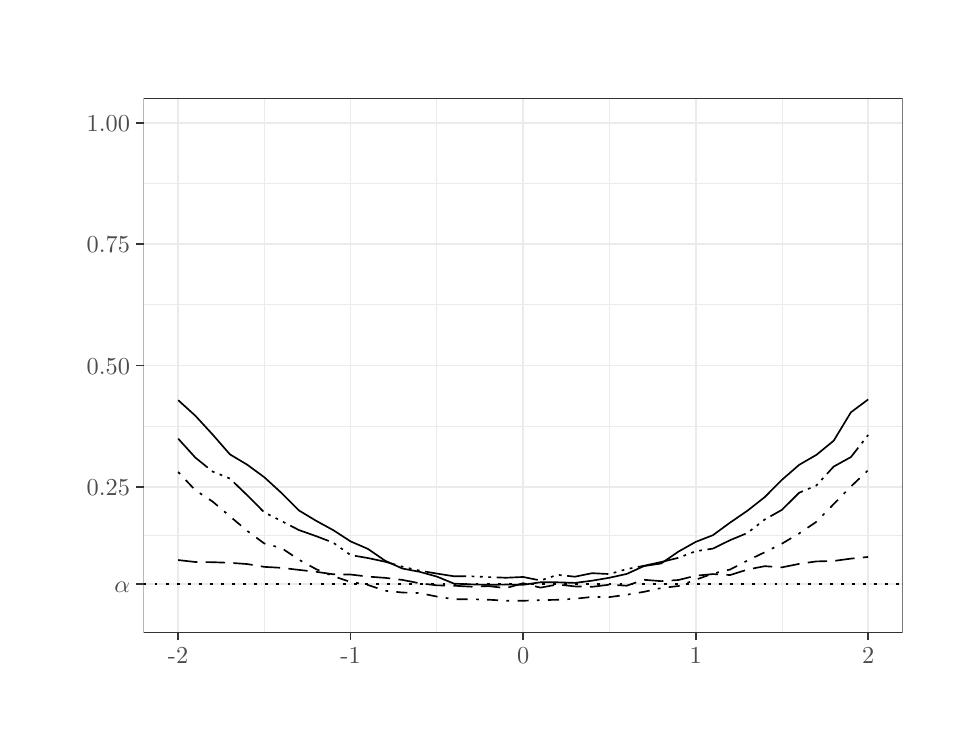
\begin{tikzpicture}[x=1pt,y=1pt]
\definecolor{fillColor}{RGB}{255,255,255}
\path[use as bounding box,fill=fillColor,fill opacity=0.00] (0,0) rectangle (325.21,252.94);
\begin{scope}
\path[clip] (  0.00,  0.00) rectangle (325.21,252.94);
\definecolor{drawColor}{RGB}{255,255,255}
\definecolor{fillColor}{RGB}{255,255,255}

\path[draw=drawColor,line width= 0.6pt,line join=round,line cap=round,fill=fillColor] (  0.00,  0.00) rectangle (325.21,252.94);
\end{scope}
\begin{scope}
\path[clip] ( 41.90, 34.26) rectangle (316.18,227.38);
\definecolor{fillColor}{RGB}{255,255,255}

\path[fill=fillColor] ( 41.90, 34.26) rectangle (316.18,227.38);
\definecolor{drawColor}{gray}{0.92}

\path[draw=drawColor,line width= 0.3pt,line join=round] ( 41.90, 69.37) --
	(316.18, 69.37);

\path[draw=drawColor,line width= 0.3pt,line join=round] ( 41.90,108.87) --
	(316.18,108.87);

\path[draw=drawColor,line width= 0.3pt,line join=round] ( 41.90,152.76) --
	(316.18,152.76);

\path[draw=drawColor,line width= 0.3pt,line join=round] ( 41.90,196.65) --
	(316.18,196.65);

\path[draw=drawColor,line width= 0.3pt,line join=round] ( 85.53, 34.26) --
	( 85.53,227.38);

\path[draw=drawColor,line width= 0.3pt,line join=round] (147.87, 34.26) --
	(147.87,227.38);

\path[draw=drawColor,line width= 0.3pt,line join=round] (210.21, 34.26) --
	(210.21,227.38);

\path[draw=drawColor,line width= 0.3pt,line join=round] (272.55, 34.26) --
	(272.55,227.38);

\path[draw=drawColor,line width= 0.6pt,line join=round] ( 41.90, 51.81) --
	(316.18, 51.81);

\path[draw=drawColor,line width= 0.6pt,line join=round] ( 41.90, 86.93) --
	(316.18, 86.93);

\path[draw=drawColor,line width= 0.6pt,line join=round] ( 41.90,130.82) --
	(316.18,130.82);

\path[draw=drawColor,line width= 0.6pt,line join=round] ( 41.90,174.71) --
	(316.18,174.71);

\path[draw=drawColor,line width= 0.6pt,line join=round] ( 41.90,218.60) --
	(316.18,218.60);

\path[draw=drawColor,line width= 0.6pt,line join=round] ( 54.37, 34.26) --
	( 54.37,227.38);

\path[draw=drawColor,line width= 0.6pt,line join=round] (116.70, 34.26) --
	(116.70,227.38);

\path[draw=drawColor,line width= 0.6pt,line join=round] (179.04, 34.26) --
	(179.04,227.38);

\path[draw=drawColor,line width= 0.6pt,line join=round] (241.38, 34.26) --
	(241.38,227.38);

\path[draw=drawColor,line width= 0.6pt,line join=round] (303.71, 34.26) --
	(303.71,227.38);
\definecolor{drawColor}{RGB}{0,0,0}

\path[draw=drawColor,line width= 0.6pt,dash pattern=on 1pt off 3pt on 4pt off 3pt ,line join=round] ( 54.37, 92.40) --
	( 60.60, 85.77) --
	( 66.83, 81.70) --
	( 73.07, 76.39) --
	( 79.30, 71.13) --
	( 85.53, 66.53) --
	( 91.77, 64.88) --
	( 98.00, 60.70) --
	(104.24, 57.26) --
	(110.47, 54.73) --
	(116.70, 52.66) --
	(122.94, 51.57) --
	(129.17, 49.46) --
	(135.40, 48.83) --
	(141.64, 48.65) --
	(147.87, 47.36) --
	(154.10, 46.41) --
	(160.34, 46.41) --
	(166.57, 46.23) --
	(172.81, 45.88) --
	(179.04, 45.85) --
	(185.27, 46.09) --
	(191.51, 46.20) --
	(197.74, 46.58) --
	(203.97, 47.25) --
	(210.21, 47.18) --
	(216.44, 48.02) --
	(222.68, 49.08) --
	(228.91, 50.45) --
	(235.14, 51.18) --
	(241.38, 53.43) --
	(247.61, 55.68) --
	(253.84, 57.15) --
	(260.08, 60.38) --
	(266.31, 63.37) --
	(272.55, 66.49) --
	(278.78, 70.18) --
	(285.01, 74.39) --
	(291.25, 80.78) --
	(297.48, 87.14) --
	(303.71, 93.04);

\path[draw=drawColor,line width= 0.6pt,dash pattern=on 15pt off 2pt on 1pt off 2pt on 1pt off 2pt on 1pt off 2pt ,line join=round] ( 54.37,104.45) --
	( 60.60, 97.57) --
	( 66.83, 92.54) --
	( 73.07, 90.02) --
	( 79.30, 84.01) --
	( 85.53, 77.76) --
	( 91.77, 74.64) --
	( 98.00, 71.41) --
	(104.24, 69.20) --
	(110.47, 66.81) --
	(116.70, 62.35) --
	(122.94, 61.29) --
	(129.17, 59.96) --
	(135.40, 58.17) --
	(141.64, 56.73) --
	(147.87, 55.68) --
	(154.10, 54.69) --
	(160.34, 54.69) --
	(166.57, 54.41) --
	(172.81, 54.17) --
	(179.04, 54.45) --
	(185.27, 53.18) --
	(191.51, 55.22) --
	(197.74, 54.55) --
	(203.97, 55.82) --
	(210.21, 55.50) --
	(216.44, 57.29) --
	(222.68, 58.49) --
	(228.91, 59.86) --
	(235.14, 61.37) --
	(241.38, 63.75) --
	(247.61, 64.70) --
	(253.84, 67.76) --
	(260.08, 70.35) --
	(266.31, 75.20) --
	(272.55, 78.71) --
	(278.78, 84.89) --
	(285.01, 87.52) --
	(291.25, 94.34) --
	(297.48, 97.78) --
	(303.71,105.75);

\path[draw=drawColor,line width= 0.6pt,dash pattern=on 7pt off 3pt ,line join=round] ( 54.37, 60.56) --
	( 60.60, 59.86) --
	( 66.83, 59.79) --
	( 73.07, 59.57) --
	( 79.30, 59.12) --
	( 85.53, 58.10) --
	( 91.77, 57.75) --
	( 98.00, 57.01) --
	(104.24, 56.31) --
	(110.47, 55.43) --
	(116.70, 55.33) --
	(122.94, 54.59) --
	(129.17, 54.13) --
	(135.40, 53.39) --
	(141.64, 52.17) --
	(147.87, 51.43) --
	(154.10, 51.29) --
	(160.34, 50.94) --
	(166.57, 51.15) --
	(172.81, 50.41) --
	(179.04, 52.20) --
	(185.27, 50.59) --
	(191.51, 51.74) --
	(197.74, 51.04) --
	(203.97, 50.90) --
	(210.21, 51.67) --
	(216.44, 51.29) --
	(222.68, 53.43) --
	(228.91, 52.94) --
	(235.14, 53.36) --
	(241.38, 54.90) --
	(247.61, 55.50) --
	(253.84, 55.15) --
	(260.08, 57.12) --
	(266.31, 58.35) --
	(272.55, 57.92) --
	(278.78, 59.19) --
	(285.01, 60.07) --
	(291.25, 60.24) --
	(297.48, 61.08) --
	(303.71, 61.68);

\path[draw=drawColor,line width= 0.6pt,line join=round] ( 54.37,118.35) --
	( 60.60,112.70) --
	( 66.83,105.92) --
	( 73.07, 98.76) --
	( 79.30, 95.04) --
	( 85.53, 90.47) --
	( 91.77, 84.75) --
	( 98.00, 78.50) --
	(104.24, 74.74) --
	(110.47, 71.34) --
	(116.70, 67.30) --
	(122.94, 64.60) --
	(129.17, 60.31) --
	(135.40, 57.50) --
	(141.64, 56.31) --
	(147.87, 54.59) --
	(154.10, 52.03) --
	(160.34, 51.78) --
	(166.57, 51.60) --
	(172.81, 51.71) --
	(179.04, 51.64) --
	(185.27, 52.52) --
	(191.51, 52.52) --
	(197.74, 52.31) --
	(203.97, 53.11) --
	(210.21, 54.17) --
	(216.44, 55.54) --
	(222.68, 58.38) --
	(228.91, 59.33) --
	(235.14, 63.61) --
	(241.38, 67.12) --
	(247.61, 69.55) --
	(253.84, 74.11) --
	(260.08, 78.39) --
	(266.31, 83.28) --
	(272.55, 89.56) --
	(278.78, 94.97) --
	(285.01, 98.58) --
	(291.25,103.68) --
	(297.48,113.96) --
	(303.71,118.60);

\path[draw=drawColor,line width= 0.6pt,dash pattern=on 1pt off 3pt ,line join=round] ( 41.90, 51.81) -- (316.18, 51.81);
\definecolor{drawColor}{gray}{0.20}

\path[draw=drawColor,line width= 0.6pt,line join=round,line cap=round] ( 41.90, 34.26) rectangle (316.18,227.38);
\end{scope}
\begin{scope}
\path[clip] (  0.00,  0.00) rectangle (325.21,252.94);
\definecolor{drawColor}{gray}{0.30}

\node[text=drawColor,anchor=base east,inner sep=0pt, outer sep=0pt, scale=  0.88] at ( 36.95, 48.78) {$\alpha$};

\node[text=drawColor,anchor=base east,inner sep=0pt, outer sep=0pt, scale=  0.88] at ( 36.95, 83.90) {$0.25$};

\node[text=drawColor,anchor=base east,inner sep=0pt, outer sep=0pt, scale=  0.88] at ( 36.95,127.79) {$0.50$};

\node[text=drawColor,anchor=base east,inner sep=0pt, outer sep=0pt, scale=  0.88] at ( 36.95,171.68) {$0.75$};

\node[text=drawColor,anchor=base east,inner sep=0pt, outer sep=0pt, scale=  0.88] at ( 36.95,215.57) {$1.00$};
\end{scope}
\begin{scope}
\path[clip] (  0.00,  0.00) rectangle (325.21,252.94);
\definecolor{drawColor}{gray}{0.20}

\path[draw=drawColor,line width= 0.6pt,line join=round] ( 39.15, 51.81) --
	( 41.90, 51.81);

\path[draw=drawColor,line width= 0.6pt,line join=round] ( 39.15, 86.93) --
	( 41.90, 86.93);

\path[draw=drawColor,line width= 0.6pt,line join=round] ( 39.15,130.82) --
	( 41.90,130.82);

\path[draw=drawColor,line width= 0.6pt,line join=round] ( 39.15,174.71) --
	( 41.90,174.71);

\path[draw=drawColor,line width= 0.6pt,line join=round] ( 39.15,218.60) --
	( 41.90,218.60);
\end{scope}
\begin{scope}
\path[clip] (  0.00,  0.00) rectangle (325.21,252.94);
\definecolor{drawColor}{gray}{0.20}

\path[draw=drawColor,line width= 0.6pt,line join=round] ( 54.37, 31.51) --
	( 54.37, 34.26);

\path[draw=drawColor,line width= 0.6pt,line join=round] (116.70, 31.51) --
	(116.70, 34.26);

\path[draw=drawColor,line width= 0.6pt,line join=round] (179.04, 31.51) --
	(179.04, 34.26);

\path[draw=drawColor,line width= 0.6pt,line join=round] (241.38, 31.51) --
	(241.38, 34.26);

\path[draw=drawColor,line width= 0.6pt,line join=round] (303.71, 31.51) --
	(303.71, 34.26);
\end{scope}
\begin{scope}
\path[clip] (  0.00,  0.00) rectangle (325.21,252.94);
\definecolor{drawColor}{gray}{0.30}

\node[text=drawColor,anchor=base,inner sep=0pt, outer sep=0pt, scale=  0.88] at ( 54.37, 23.25) {-2};

\node[text=drawColor,anchor=base,inner sep=0pt, outer sep=0pt, scale=  0.88] at (116.70, 23.25) {-1};

\node[text=drawColor,anchor=base,inner sep=0pt, outer sep=0pt, scale=  0.88] at (179.04, 23.25) {0};

\node[text=drawColor,anchor=base,inner sep=0pt, outer sep=0pt, scale=  0.88] at (241.38, 23.25) {1};

\node[text=drawColor,anchor=base,inner sep=0pt, outer sep=0pt, scale=  0.88] at (303.71, 23.25) {2};
\end{scope}
\end{tikzpicture}
